% !TEX root = marvin.tex
\begin{figure*}[t]
\begin{center}
\iflatexml
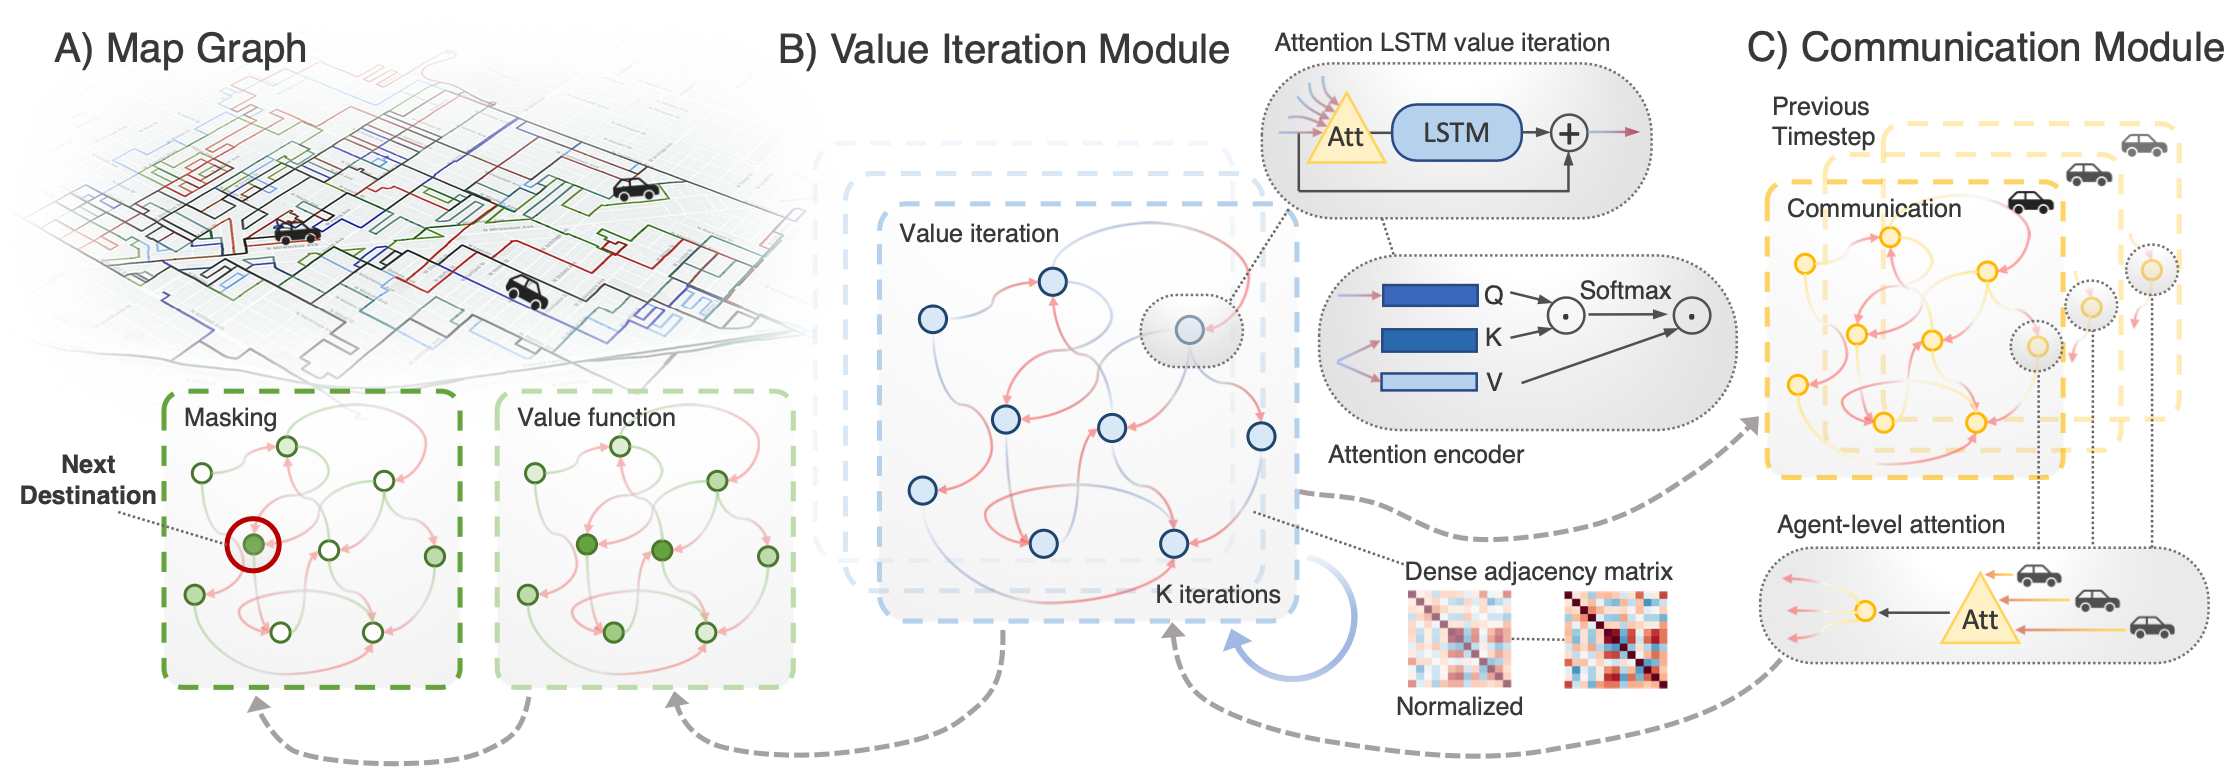
\includegraphics[width=6\textwidth]{figs/model2.png}
\else
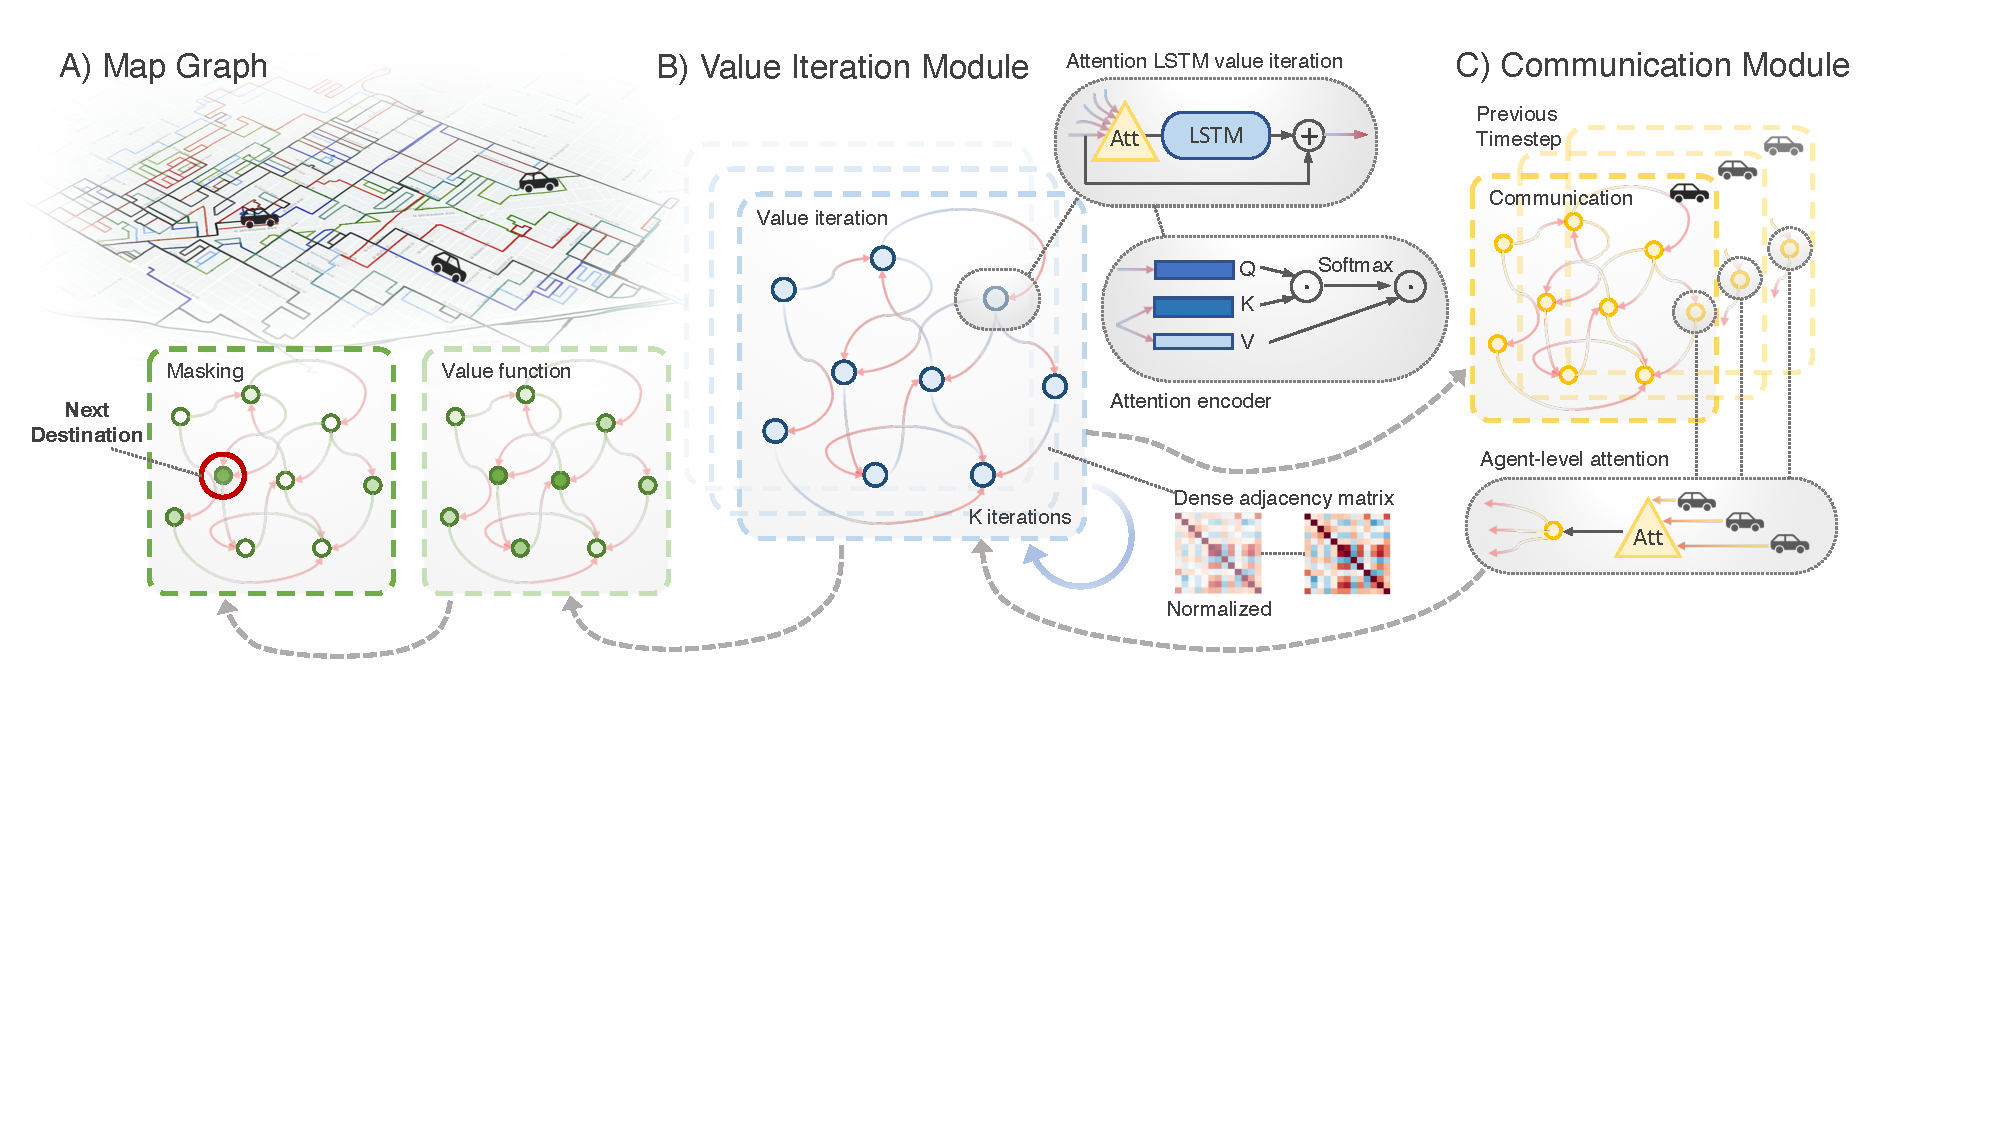
\includegraphics[width=0.975\textwidth,trim={0 7.5cm 2cm 0.5cm},clip]{figs/model2.pdf}
\fi
\vspace{-0.15in}
\caption{\textbf{Our proposed multi-agent routing value iteration network}:
\textbf{A)} The map is represented as a graph and each node has some local observation features;
\textbf{B)} Each agent operates its own value iteration network. It uses an attention-based LSTM on
each graph node to exchange information. The LSTM runs for $k$ iterations and can be decoded into a
value function for selecting next destination. \textbf{C)} Inter-agent communication is implemented
with an attention mechanism over all the incoming messages, and the output is fed as additional
channels of inputs to the value iteration module.}
\label{fig:mainfig}
\end{center}
\vspace{-0.2in}
\end{figure*}